% LaTeX file for resume 
% This file uses the resume document class (res.cls)

\documentclass{res}
\usepackage[utf8]{inputenc}
\usepackage{hyperref}
\usepackage{graphicx}
\usepackage{float}
\usepackage{wrapfig}

%\usepackage{helvetica} % uses helvetica postscript font (download helvetica.sty)
%\usepackage{newcent}   % uses new century schoolbook postscript font 
\newsectionwidth{0pt}  % So the text is not indented under section headings
\usepackage{fancyhdr}  % use this package to get a 2 line header
\renewcommand{\headrulewidth}{0pt} % suppress line drawn by default by fancyhdr
\setlength{\headheight}{24pt} % allow room for 2-line header
\setlength{\headsep}{24pt}  % space between header and text
\setlength{\headheight}{24pt} % allow room for 2-line header
\pagestyle{fancy}     % set pagestyle for document
\rhead{ {\it Mauro Ezequiel Bender}\\{\it p. \thepage} } % put text in header (right side)
\cfoot{}                                     % the foot is empty
\topmargin=-0.5in % start text higher on the page

\begin{document}
\thispagestyle{empty} % this page has no header  

\begin{tabular}{l r}
  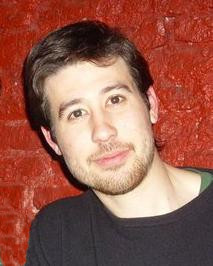
\includegraphics[bb=0 0 213 266,scale=0.35,keepaspectratio=true]{./yo.jpg} &
  \raisebox{1,1cm}[1,1cm][0cm]{
  \parbox{360px}{\raggedleft 
		\textbf{\Large Mauro Ezequiel Bender} \\
		Dragones 2717, González Catán \\
		Buenos Aires \\
		Cel: (011) 15-3911-4033  \\
		Email: \href{mailto:maurobender@gmail.com}{maurobender@gmail.com} \\
		\url{http://ar.linkedin.com/in/maurobender} \\
		\vspace{40px}
		}
	}
\end{tabular}

\begin{resume}
 
\section{\centerline{OBJETIVO}}
\begin{center}
\vspace{-40pt} 
\line(1,0){470}
\end{center}

% provide vertical space between section title and contents
Busco una posición como desarrollador web para frontend o backend en la que pueda aplicar mis conocimientos,
en un ambiente agradable, y que me permita a la vez aprender sobre nuevas tecnologías y crecer en
el campo profesional. 
 
\vspace{0.2in}
\section{\centerline{EDUCACIÓN}} 
\begin{center}
\vspace{-40pt} 
\line(1,0){470}
\end{center}


{\sl Licenciatura en Ciencias de la computación} \\
Universidad de Buenos Aires \hspace{0.2in}  \hfill 2007 - Actualidad 
 
{\sl Técnico en electrónica} \\ % \sl will be bold italic in
					 % New Century Schoolbook (or
					 % any postscript font) and
					 % just slanted in Computer
					 % Modern (default) font
Escuela de Educación Técnica Nº6, Isidro Casanova      \hfill    2003 - 2005

\vspace{0.2in}
\section{\centerline{IDIOMAS}}
\begin{center}
\vspace{-40pt} 
\line(1,0){470}
\end{center}

\begin{itemize} \itemsep -2pt
 \item Español (Nativo)
 \item Inglés (Intermedio)
 \item Francés (Básico)
 \item Japonés (Básico)
\end{itemize}

\vspace{0.2in} 
\section{\centerline{CONOCIMIENTOS }}
\begin{center}
\vspace{-40pt} 
\line(1,0){470}
\end{center}

\begin{itemize} \itemsep -2pt
	\item Linux
	\item PHP
	\item MySQL
	\item JavaScript
	\item JQuery, JQuery UI
	\item Frameworks MVC: CakePHP (PHP), Yii (PHP), Backbone.js (JavaScript)
	\item HTML (4/5)
	\item CSS (2/3)
	\item Sistemas de control de versiones: SVN, Git.
	\item C, C++
	\item Qt, Gtk
	\item Java
	\item Doxygen, \LaTeX
\end{itemize}
  
\vspace{0.2in} 
\section{\centerline{EXPERIENCIA PROFESIONAL}} 
\begin{center}
\vspace{-40pt} 
\line(1,0){470}
\end{center}

{\sl Desarrollador Web} \hfill        Marzo 2009 - Actualidad \\
Insite Latin America, Capital Federal   \hfill \url{www.insite-la.com}
	\begin{itemize} \itemsep -2pt % reduce space between items
		\item Desarrollo de diversos sitios web para las diferentes cuentas de la agencia,
		como HP, P\&G y 3M. Dentro de estas tareas se pueden destacar:
		\begin{itemize} \itemsep -2pt % reduce space between items
			\item Mantenimiento de las tiendas online para HP Argentina y Latam y para la tienda
			de 3M Colombia.
			\item Desarrollo de una red social para odontólogos de 3M Colombia utilizando PHP (con CakePHP Framework)
			y MySQL: \url{www.espertiseclub.com}.
			\item Desarrollo de un sitio destinado a odontólogos, auxiliares y estudiantes de odontología de 3M
			Colombia utilizando PHP (con CakePHP Framework) y MySQL: \url{www.esperiencias.com.co}.
			\item Desarrollo y mantenimiento de una tienda en línea para 3M Colombia utilizando PHP (con Yii Framework)
			y MySQL: \url{www.compra3m.com.co}. En este proyecto en particular se desarrollaron extensiones y
			componentes adicionales para el framework utilizado con el fin de crear un módulo de conexión vía
			FTP con el servidor de logística, con el cual debían sincronizarse el stock de los productos y el
			estado de las órdenes.
		\end{itemize}
		\item Matenimiento y modificaciones en sitios web ya existentes desarrollados con diferentes tecnologías como
		PHP, MySQL, Java (Struts) y PostgreSQL.
		\item Asesoramiento y soporte al equipo de maquetadores de la agencia sobre cuestiones relacionadas con código
		del lado del cliente (JavaScript, JQuery, MooTools) en páginas estáticas y para contenido cargado mediante CMS.
	\end{itemize}
\textbf{Referencias}: Mara Avila (Project Manager): \href{mailto:avilamara@hotmail.com}{avilamara@hotmail.com} / 15.5954.6272

\vspace{0.2in} 
\section{\centerline{PROYECTOS PERSONALES}} 
\begin{center}
\vspace{-40pt} 
\line(1,0){470}
\end{center}

{\sl Desarrollador Web \& Co-Founder} \hfill        Julio 2011 - Actualidad \\
Vitbok.com   \hfill \url{www.vitbok.com} \\ \\
\textbf{Vitbok.com} es una red social que simula un diario personal. Fue desarrollado en PHP siguiendo el
patrón de diseño MVC, usando \href{http://www.yiiframework.com/}{Yii Framework} y MySQL. Del lado del cliente el código JavaScript
también fue organizado siguiendo un patrón MVC usando \href{http://backbonejs.org/}{Backbone.js} (pero sin la utilización de controladores).
Además de la aplicación principal se dispone de un módulo encargado de proporcionar una API REST
(interna) para todas las operaciones que se realizan mediante Ajax.

\subsection{{\small OTROS PROYECTOS}}
\vspace{-0.2in}
Proyectos en Sourceforge: \url{https://sourceforge.net/users/maurobender} \\
Proyectos en GitHub: \url{https://github.com/maurobender}

\section{\centerline{INFORMACIÓN PERSONAL}}
\begin{center}
\vspace{-40pt} 
\line(1,0){470}
\end{center}

% provide vertical space between section title and contents
\begin{itemize} \itemsep -2pt % reduce space between items
		\item Estado Civil: Soltero.
		\item Nacionalidad: Argentino.
		\item Edad: 25 años.
		\item DNI: 33.613.217.
	\end{itemize}
 
% \vspace{0.2in}
% \section{\centerline{INTERESES}} 
% \vspace{-5pt} 
% \begin{center}
% Idiomas, Nuevas tecnologías, Fotografía, Literatura
% 
% \end{center} 
 
\end{resume} 
\end{document}













